Имея склейку, мы можем охарактеризовать двумерное многообразие словом. Начиная с какой-то точки будем идти по границе склейки и выписывать встречающиеся буквы (выше обозначалось цветом, но это было только для наглядности (да кого я обманываю, мне просто было лень заморачиваться ещё и над гарнитурами)). Если направление стрелки совпадает с направлением обхода, то записываем букву как есть, иначе — записываем как бы в минус первой степени (см.рис.\ref{fig:c10.2}).

\begin{figure}[H]
    \centering
    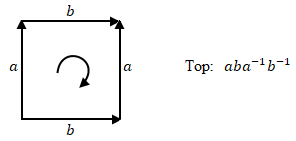
\includegraphics[scale=1]{images/c10.2.png}
    \caption{Склейка тора из квадрата.}
    \label{fig:c10.2}
\end{figure}

Слово задаётся неоднозначно, но по нему можно однозначно построить многообразие.

Можно обобщить данный метод на любой $2k$-угольник, у которого стороны помечены буквами и каждая буква встречается ровно 2 раза.

В результате склейки такого многоугольника мы получим двумерное многообразие (после склейки у каждой точки окрестность будет гомеоморфна диску).

Далее наша задача будет состоять в том, чтобы классифицировать все компактные связные двумерные многообразия с помощью таких слов. Итак,

\begin{theorem}
    Любое связное компактное двумерное многообразие $X$ гомеоморфно многообразию, полученному склейкой сторон многоугольника по одному из следующих слов:
    \begin{enumerate}
        \item $aa^{-1}$;
        \item $a_1b_1a_1^{-1}b_1^{-1}\dots a_n b_n a_n^{-1} b_n^{-1}, \ n \geqslant 1$;
        \item $a_1 a_1 a_2 a_2 \dots a_m a_m, \ m \geqslant 1$.
    \end{enumerate}
\end{theorem} 
Прежде чем доказывать данную теорему, введём следующие определения:
\begin{definition}
    \textit{Топологический треугольник в многообразии $X$} — некоторое подмножество, которое гомеоморфно треугольнику на плоскости со структурой вершины-стороны (см.рис.\ref{fig:c10.1})
\end{definition} 
\begin{definition}
    \textit{Триангуляция двумерного многообразия $X$} — это представление $X$ в виде объединения топологических треугольников с условием на их пересечение: два топологических треугольника либо не пересекаются, либо пересекаются по вершине, либо пересекаются по стороне.
\end{definition} 

\begin{figure}[htbp]
    \centering
    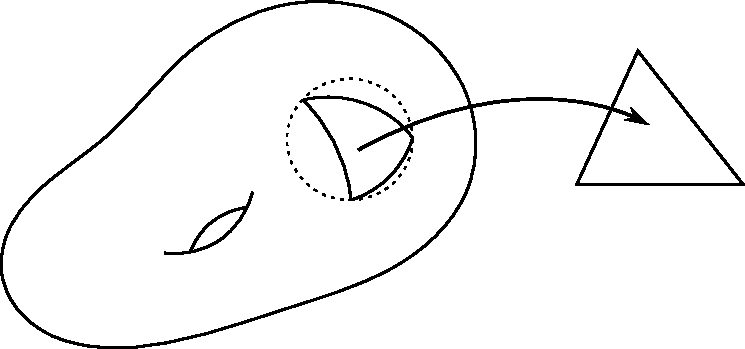
\includegraphics[scale=1]{images/c10.1.pdf}
    \caption{К определению триангуляции.}
    \label{fig:c10.1}
\end{figure}

\begin{proof}
    Мы будем классифицировать такие двумерные многообразия без края, для которых существует конечная триангуляция.
    
    \textbf{Первый этап доказательства.} Существование многоугольника, задающего многообразие.
    Рассмотрим на $X$ конечную триангуляцию. Разрежем $X$ на треугольники, помечая их стороны разными буквами и стрелками, чтобы получить набор треугольников, каждая сторона которых помечена буквой и выбрано направление, причём каждая буква будет встречаться ровно два раза.

    \begin{figure}[ht]
        \centering
        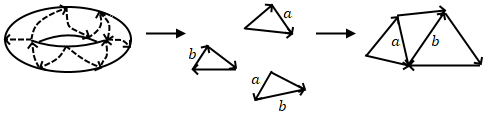
\includegraphics[scale=1]{images/c10.3.png}
        \caption{Построение многоугольника из двумерного многообразия.}
        \label{fig:c10.3}
    \end{figure}

    Поскольку $X$ связно, у нас будет конечное количество треугольников (действительно, если мы не можем приклеить треугольник, тогда мы получили многоугольник, на границе которого каждая буква встречается ровно два раза — склеив соответствующие стороны, получим связное двумерное многообразие, а из оставшихся склеим что-то ещё — противоречие с изначальной связностью множества), которые мы будем собирать вместе, приклеивая к уже полученному многоугольнику. В результате получим многоугольник, результатом склейки сторон которого будет многообразие $X$.

    Теперь нам надо поменять слово, которое задаёт этот многоугольник таким образом, чтобы привести его к одному из канонических видов.

    \textbf{Второй этап доказательства.} Алгоритм изменения слова до канонического вида.
    \begin{enumerate}
        \item Вычёркивание фрагмента вида $\dots a a^{-1} \dots$:
        Если в слове есть фрагмент $\dots a a^{-1} \dots$ (причём $a a^{-1}$ — это не всё слово), то вычёркиваем его. Действительно, после склейки фрагмент слова $aa^{-1}$ пропадёт 

        \begin{figure}[ht]
            \centering
            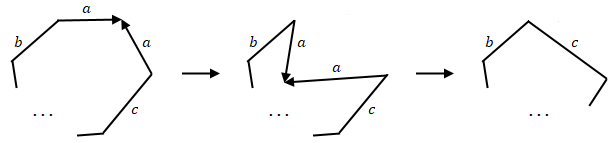
\includegraphics[scale=0.7]{images/c10.4.png}
            \caption{Вычёркивание фрагмента вида $\dots a a^{-1} \dots$.}
            \label{fig:c10.4}
        \end{figure}

        \item Приведение к одной вершине: 
        Пометим все вершины многоугольника буквами ($A,B, \dots$), которые соответствуют этим вершинам после склейки. Пусть не все вершины многоугольника склеиваются в одну, тогда есть сторона многоугольника, концы которой не склеиваются, то есть принадлежат разным классам. Пометим эту сторону буквой $a$. Тогда соседняя сторона может быть помечена буквой $b \neq a$ (случай $\dots aa \dots$ невозможен, потому что мы предположили, что вершины $A$ и $B$ не склеиваются, а случай $\dots aa^{-1} \dots$ исключён по первому пункту).

        Найдём в многоугольнике вторую сторону, помеченную буквой $b$. Теперь отрежем помеченный треугольник и приклеим его к стороне $b$ так, как показано на рис.\ref{fig:c10.5}.

        \begin{figure}[ht]
            \centering
            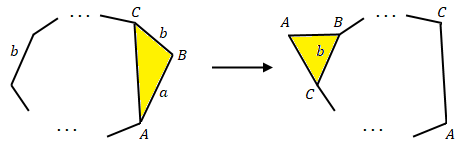
\includegraphics[scale=0.7]{images/c10.5.png}
            \caption{Уменьшение вершин класса $B$.}
            \label{fig:c10.5}
        \end{figure}

        В результате вершин класса $B$ стало на одну меньше, а вершин класса $A$ на одну больше (несложно понять, что если вершина какого-то класса останется одна, то склеятся рёбра, подходящие к этой вершине, и она уничтожится). Будем повторять данную операцию до тех пор, пока не останется один класс вершин, то есть все вершины многогранника будут склеиваться в одну.

        \item Собираем вместе пары вида $\dots a \dots a \dots$. Если на границе многоугольника есть две стороны, помеченные одинаковой буквой так, что направление обхода сторон одинаковое относительно обхода границы многоугольника, то разрежем многоугольник так, как показано на рис.\ref{fig:c10.6} и склеим по стороне $a$.
        
        \begin{figure}[ht]
            \centering
            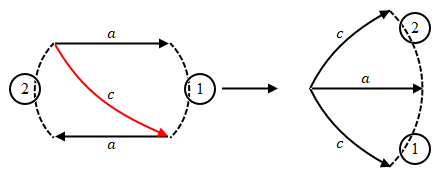
\includegraphics[scale=0.7]{images/c10.6.png}
            \caption{Склейка многоугольника по стороне $a$.}
            \label{fig:c10.6}
        \end{figure}

        Теперь два ребра, помеченные одной буквой, стоят рядом. Будем совершать эту операцию до тих пор, пока в слове есть две одинаковые буквы (в одинаковых степенях), не стоящие рядом.

        Если на этом этапе мы получили слово вида $a_1 a_1 a_2 a_2 \dots a_m a_m$, то пришли к одному из канонических видов. Иначе:

        \item Собираем вместе четвёрки $\dots a \dots b \dots a^{-1} \dots b^{-1} \dots$.
        Если после шага 2 есть буквы, входящие в слово как $\dots b \dots$ и $\dots b^{-1} \dots$, тогда две стороны, помеченные одинаковой буквой, расположенные так, как показано на рис.\ref{fig:c10.7}, лежащие в разных частях (есть ещё пара $a$ и $a^{-1}$, причём в слове они встречаются так: $\dots b \dots a \dots b^{-1} \dots a^{-1} \dots$).

        \begin{figure}[ht]
            \centering
            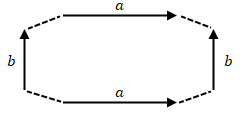
\includegraphics[scale=0.7]{images/c10.7.png}
            \caption{Четвёрка $b a b^{-1} a^{-1}$.}
            \label{fig:c10.7}
        \end{figure}

        Действительно, не может быть так, чтобы стороны из частей, на которые границу многоугольника делят $b$ и $b^{-1}$, склеивались только между собой — в этом случае вершины из этих частей склеивались бы только между собой, а это противоречит шагу 2 (приведение к одной вершине).

        При этом рёбра, помеченные буквой $a$, расположены так, как показано на рис.\ref{fig:c10.7} — если у одной из стрелок поменять направление, то получим два ребра, которые направлены в одну сторону относительно обхода границы многоугольника, а это противоречит шагу 3.

        Собираем четвёрки $\dots a \dots b \dots a^{-1} \dots b^{-1} \dots$ вместе следующим образом. Сначала проведём разрез $x$ как показано на рис.\ref{fig:c10.8} и склеим по стороне $b$.

        \begin{figure}[ht]
            \centering
            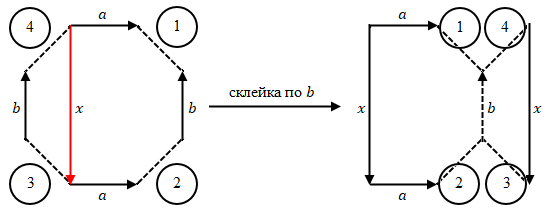
\includegraphics[scale=0.7]{images/c10.8.png}
            \caption{Склейка многоугольника по стороне $b$.}
            \label{fig:c10.8}
        \end{figure}

        Теперь проведём разрез $y$ и склеим по стороне $a$ (см.рис.\ref{fig:c10.9}).

        \begin{figure}[ht]
            \centering
            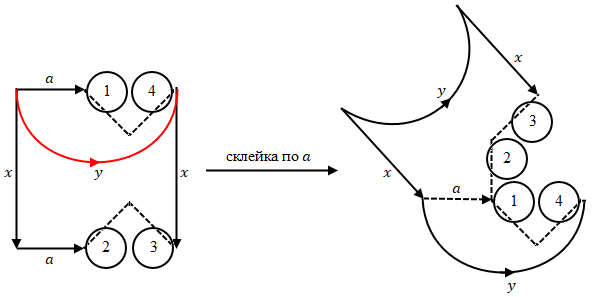
\includegraphics[scale=0.7]{images/c10.9.png}
            \caption{Склейка многоугольника по стороне $a$.}
            \label{fig:c10.9}
        \end{figure}

        Получаем $y^{-1}x^{-1}yx$. Переобозначая направление стрелок, получим что требовалось. Фрагменты 1, 2, 3, 4 направлены так же, как и до переклеек, что гарантирует нам то, что при переклейках мы ничего не испортили (не нужно запускать шаг 2).

        После этого шага алгоритма либо мы получили канонический вид $$a_1 b_1 a_1^{-1} b_1^{-1} \dots a_n b_n a_n^{-1} b_n^{-1},$$ либо в полученном слове есть фрагменты вида $$a_1 b_1 a_1^{-1} b_1^{-1} \dots a_n b_n a_n^{-1} b_n^{-1}$$ и $$a_1 a_1 a_2 a_2 \dots a_m a_m,$$ причём они стоят рядом.

        \item Если в слове есть фрагменты вида $\dots aa \dots$ и $\dots xyx^{-1}y^{-1} \dots$.
        Проведём разрез $b$ и склеим по стороне $a$ (см.рис.\ref{fig:c10.10}).

        \begin{figure}[H]
            \centering
            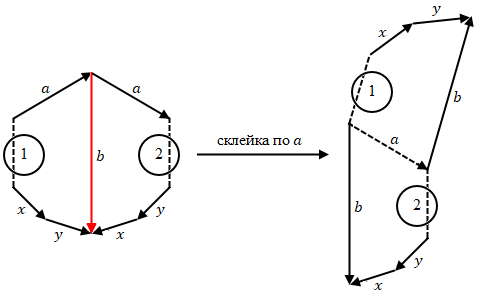
\includegraphics[scale=0.7]{images/c10.10.png}
            \caption{Склейка многоугольника по $a$.}
            \label{fig:c10.10}
        \end{figure}

        Теперь проведём разрез $p$ и склеим по стороне $x$ (см.рис.\ref{fig:c10.11}).

        \begin{figure}[h]
            \centering
            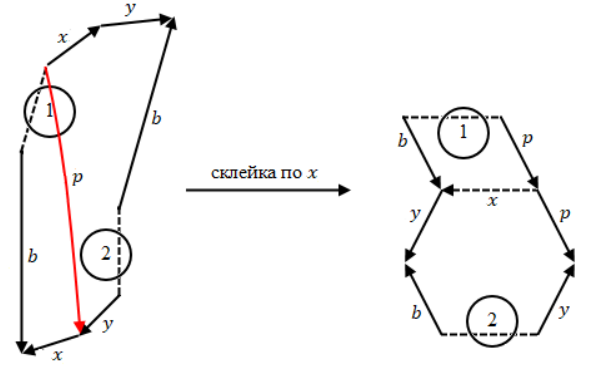
\includegraphics[scale=0.5]{images/c10.11.png}
            \caption{Склейка многоугольника по стороне $x$.}
            \label{fig:c10.11}
        \end{figure}

        Далее проведём разрез $q$ и склеим по стороне $y$ (см.рис.\ref{fig:c10.12}).

        \begin{figure}[h]
            \centering
            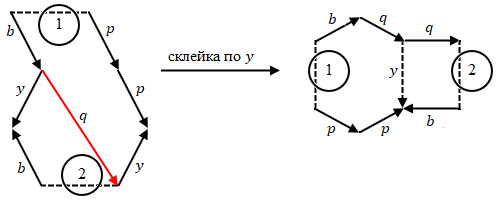
\includegraphics[scale=0.7]{images/c10.12.png}
            \caption{Склейка многоугольника по стороне $y$.}
            \label{fig:c10.12}
        \end{figure}

        Наконец сделаем разрез $z$ и склеим по стороне $b$ (см.рис.\ref{fig:c10.13}).

        \begin{figure}[h]
            \centering
            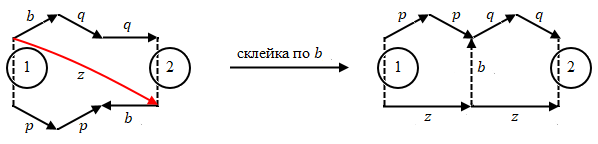
\includegraphics[scale=0.7]{images/c10.13.png}
            \caption{Склейка многоугольника по стороне $b$.}
            \label{fig:c10.13}
        \end{figure}

        Вместо пары фрагментов $\dots aa \dots$ и $\dots xyx^{-1}y^{-1} \dots$ возникли фрагменты $\dots zz \dots$ и $\dots ppqq \dots$. Таким образом, пока есть пары фрагментов вида $\dots aa \dots$ и $\dots xyx^{-1}y^{-1} \dots$, мы можем совершать эту операцию, после которой фрагмент $xyx^{-1}y^{-1}$ уничтожается. В результате мы придём к каноническому слову $a_1a_1a_2a_2 \dots a_ma_m$.
    \end{enumerate}
\end{proof} 

\begin{remark}
    Многообразия, принадлежащие различным сериям, не гомеоморфны между собой. Также не гомеоморфны между собой многообразия из одной серии при различных $n$.
\end{remark}